%!Tex Program = xelatex
% -*-coding: utf-8 -*-
%  \author{初砚硕}
\def\usewhat{xelatex} % 定义编译方式 pdflatex, dvipdfmx, or xelatex____ps:只有xelatex 能使用Arial字体

\def\version{1.1} % 模板版本号

\def\xueke{Engineering} % 定义学科 Engineering, Science, Management, or Arts

\documentclass[12pt,openany,twoside]{book}

%!Tex Program = xelatex
% -*-coding: utf-8 -*-


\usepackage{graphicx}

%\usepackage[a4paper,text={162true mm,249true mm},left=24true mm,
%            head=24true mm, top=24true mm, bottom=24true mm,
%           headheight=14true mm, headsep=10true mm
%           ]{geometry}% 东北林业大学要求的宽度

%\usepackage[a4paper,]{geometry}%四周都是24mm
\usepackage[a4paper,
left=24true mm,right=24true mm, top=25true mm, bottom=23true mm,
headheight=14true mm,
headsep=7true mm,
footskip=7true mm]{geometry}% 东北林业大学要求的宽度
\usepackage{layout}


\usepackage{titlesec}               % 控制标题的宏包
\usepackage{titletoc}                   % 控制目录的宏包
\usepackage{fancyhdr}                   % fancyhdr宏包 页眉和页脚的相关定义
%\usepackage[UTF8]{ctex}
\usepackage{color}          % 支持彩色
\usepackage{amsmath}        % AMSLaTeX宏包 用来排出更加漂亮的公式
\usepackage{amssymb}
\usepackage{epsfig}         % eps图像
\usepackage[below]{placeins}%允许上一个section 的浮动图形出现在下一个section的开始部分,还提供\FloatBarrier命令,使所有未处理的浮动图形立即被处理
\usepackage{flafter}       % 使得所有浮动体不能被放置在其浮动环境之前,以免浮动体在引述它的文本之前出现.
\usepackage{multirow}       %使用Multirow宏包,使得表格可以合并多个row 格
\usepackage{booktabs}       % 表格,横的粗线;\specialrule{1pt}{0pt}{0pt}
\usepackage{longtable}      %支持跨页的表格。
\usepackage{tabularx}
\usepackage{subfigure}%支持子图 %centerlast 设置最后一行是否居中
\usepackage[subfigure]{ccaption} %支持双语标题
\usepackage[sort&compress,numbers]{natbib}% 支持引用缩写的宏包
\makeatletter
%林大的参考文献研究用波浪链接~
\def\NAT@citexnum[#1][#2]#3{%
  \NAT@reset@parser
  \NAT@sort@cites{#3}%
  \NAT@reset@citea
  \@cite{\def\NAT@num{-1}\let\NAT@last@yr\relax\let\NAT@nm\@empty
    \@for\@citeb:=\NAT@cite@list\do
    {\@safe@activestrue
     \edef\@citeb{\expandafter\@firstofone\@citeb\@empty}%
     \@safe@activesfalse
     \@ifundefined{b@\@citeb\@extra@b@citeb}{%
       {\reset@font\bfseries?}
        \NAT@citeundefined\PackageWarning{natbib}%
       {Citation `\@citeb' on page \thepage \space undefined}}%
     {\let\NAT@last@num\NAT@num\let\NAT@last@nm\NAT@nm
      \NAT@parse{\@citeb}%
      \ifNAT@longnames\@ifundefined{bv@\@citeb\@extra@b@citeb}{%
        \let\NAT@name=\NAT@all@names
        \global\@namedef{bv@\@citeb\@extra@b@citeb}{}}{}%
      \fi
      \ifNAT@full\let\NAT@nm\NAT@all@names\else
        \let\NAT@nm\NAT@name\fi
      \ifNAT@swa
       \@ifnum{\NAT@ctype>\@ne}{%
        \@citea
        \NAT@hyper@{\@ifnum{\NAT@ctype=\tw@}{\NAT@test{\NAT@ctype}}{\NAT@alias}}%
       }{%
        \@ifnum{\NAT@cmprs>\z@}{%
         \NAT@ifcat@num\NAT@num
          {\let\NAT@nm=\NAT@num}%
          {\def\NAT@nm{-2}}%
         \NAT@ifcat@num\NAT@last@num
          {\@tempcnta=\NAT@last@num\relax}%
          {\@tempcnta\m@ne}%
         \@ifnum{\NAT@nm=\@tempcnta}{%
          \@ifnum{\NAT@merge>\@ne}{}{\NAT@last@yr@mbox}%
         }{%
           \advance\@tempcnta by\@ne
           \@ifnum{\NAT@nm=\@tempcnta}{%
             \ifx\NAT@last@yr\relax
               \def@NAT@last@yr{\@citea}%
             \else
               \def@NAT@last@yr{$\sim$\NAT@penalty}%
             \fi
           }{%
             \NAT@last@yr@mbox
           }%
         }%
        }{%
         \@tempswatrue
         \@ifnum{\NAT@merge>\@ne}{\@ifnum{\NAT@last@num=\NAT@num\relax}{\@tempswafalse}{}}{}%
         \if@tempswa\NAT@citea@mbox\fi
        }%
       }%
       \NAT@def@citea
      \else
        \ifcase\NAT@ctype
          \ifx\NAT@last@nm\NAT@nm \NAT@yrsep\NAT@penalty\NAT@space\else
            \@citea \NAT@test{\@ne}\NAT@spacechar\NAT@mbox{\NAT@super@kern\NAT@@open}%
          \fi
          \if*#1*\else#1\NAT@spacechar\fi
          \NAT@mbox{\NAT@hyper@{{\citenumfont{\NAT@num}}}}%
          \NAT@def@citea@box
        \or
          \NAT@hyper@citea@space{\NAT@test{\NAT@ctype}}%
        \or
          \NAT@hyper@citea@space{\NAT@test{\NAT@ctype}}%
        \or
          \NAT@hyper@citea@space\NAT@alias
        \fi
      \fi
     }%
    }%
      \@ifnum{\NAT@cmprs>\z@}{\NAT@last@yr}{}%
      \ifNAT@swa\else
        \@ifnum{\NAT@ctype=\z@}{%
          \if*#2*\else\NAT@cmt#2\fi
        }{}%
        \NAT@mbox{\NAT@@close}%
      \fi
  }{#1}{#2}%
}%
\makeatother

\usepackage{enumitem}       %使用enumitem宏包,改变列表项的格式
\usepackage{calc}           %长度可以用+ - * / 进行计算


%%\usepackage{txfonts}
\usepackage{mathtools}

\usepackage{bm}              % 处理数学公式中的黑斜体的宏包

% 生成有书签的pdf及其开关, 该宏包应放在所有宏包的最后, 宏包之间有冲突
\def\atemp{dvipdfmx}\ifx\atemp\usewhat
\usepackage[dvipdfm,unicode,           %dvi-->pdf 生成书签
            bookmarksnumbered=true,
            bookmarksopen=true,
            colorlinks=false,
            pdfborder={0 0 1},
            citecolor=blue,
            linkcolor=red,
            anchorcolor=green,
            urlcolor=blue,
            breaklinks=true
            ]{hyperref}
\fi

\def\atemp{pdflatex}\ifx\atemp\usewhat
\usepackage{cmap}                       %pdflatex编译时,可以生成可复制、粘贴的中文PDF 文档
\usepackage[pdftex,unicode,
            %CJKbookmarks=true,
            bookmarksnumbered=true,
            bookmarksopen=true,
            colorlinks=false,
            pdfborder={0 0 1},
            citecolor=blue,
            linkcolor=red,
            anchorcolor=green,
            urlcolor=blue,
            breaklinks=true
            ]{hyperref}
\fi

\def\atempxetex{xelatex}\ifx\atempxetex\usewhat %\def\atempxetex{xelatex} main.tex中已定义;



\usepackage[xetex,
            bookmarksnumbered=true,
            bookmarksopen=true,
            colorlinks=false,
            pdfborder={0 0 1},
            citecolor=blue,
            linkcolor=red,
            anchorcolor=green,
            urlcolor=blue,
            breaklinks=true,
            naturalnames  %与algorithm2e宏包协调
            ]{hyperref}
%\usepackage{fontenc}
%xunicode xunicode Ross Moore’s xunicode package is now automatically loaded for users of both XELATEX and LuaLATEX.
\usepackage[BoldFont,SlantFont]{xeCJK}
\defaultfontfeatures{Mapping=tex-text}

\xeCJKsetemboldenfactor{1}%只对随后定义的CJK字体有效
\setCJKfamilyfont{hei}{SimHei}
\xeCJKsetemboldenfactor{4}
\setCJKfamilyfont{song}{SimSun}
\xeCJKsetemboldenfactor{1}
\setCJKfamilyfont{fs}{FangSong}
\setCJKfamilyfont{kai}{KaiTi}
\setCJKfamilyfont{li}{LiSu}
\setCJKfamilyfont{xw}{STXinwei}

\setCJKmainfont{SimSun}
\setmainfont{Times New Roman}
\setsansfont{Arial}

\newcommand{\hei}{\CJKfamily{hei}}% 黑体   (Windows自带simhei.ttf)
\newcommand{\song}{\CJKfamily{song}}    % 宋体   (Windows自带simsun.ttf)
\newcommand{\fs}{\CJKfamily{fs}}        % 仿宋体 (Windows自带simfs.ttf)
\newcommand{\kai}{\CJKfamily{kai}}      % 楷体   (Windows自带simkai.ttf)
\newcommand{\li}{\CJKfamily{li}}        % 隶书   (Windows自带simli.ttf)
\newcommand{\xw}{\CJKfamily{xw}}        % 隶书   (Windows自带simli.ttf)


\newfontfamily\arial{Arial}
\newfontfamily\timesnewroman{Times New Roman}

%
\fi

\usepackage[boxed,linesnumbered,algochapter]{algorithm2e}%\let\chapter\undefined
% 算法的宏包,注意宏包兼容性,先后顺序为float、hyperref、algorithm(2e),否则无法生成算法列表

\usepackage{setspace}%更改行距的宏包
%\usepackage{syntonly}检查语法不编译
%\syntaxonly
\usepackage{tikz}%R语言作图使用
\usepackage{xltxtra}%输出XeLaTeX
 % 引用的宏包

\graphicspath{{figures/}} %定义所有的eps文件在 figures 子目录下


\begin{document}

%!Tex Program = xelatex
% -*-coding: utf-8 -*-


\newcommand{\xiaochu}{\fontsize{36pt}{36pt}\selectfont}       % 一号, 1.倍行距
\newcommand{\yihao}{\fontsize{26pt}{26pt}\selectfont}       % 一号, 1.倍行距
\newcommand{\xiaoyi}{\fontsize{24pt}{24pt}\selectfont}      % 小一, 1.倍行距
\newcommand{\erhao}{\fontsize{22pt}{22pt}\selectfont}       % 二号, 1.倍行距
\newcommand{\xiaoer}{\fontsize{18pt}{18pt}\selectfont}      % 小二, 单倍行距
\newcommand{\sanhao}{\fontsize{16pt}{16pt}\selectfont}      % 三号, 1.倍行距
\newcommand{\xiaosan}{\fontsize{15pt}{15pt}\selectfont}     % 小三, 1.倍行距
\newcommand{\sihao}{\fontsize{14pt}{14pt}\selectfont}       % 四号, 1.0倍行距
\newcommand{\xiaosi}{\fontsize{12pt}{12pt}\selectfont}      % 小四, 1.倍行距
\newcommand{\wuhao}{\fontsize{10.5pt}{10.5pt}\selectfont}   % 五号, 单倍行距
\newcommand{\xiaowu}{\fontsize{9pt}{9pt}\selectfont}        % 小五, 单倍行距



%避免宏包 hyperref 和 arydshln 不兼容带来的目录链接失效的问题。
\def\temp{\relax}
\let\temp\addcontentsline
\gdef\addcontentsline{\phantomsection\temp}

\newcommand{\nefuEqRef}[1]{(\ref{#1})}

\makeatletter

%\gdef\hitempty{}%全局定义空,貌似没用

%\renewcommand\labelenumi{(\theenumi )} %调整列表环境为(1)

\newcommand{\mr}[1]{\mathrm{#1}} %定义新命令,用\mr来代替\mathrm

%重新定义BiChapter命令,可实现标题手动换行,但不影响目录
\def\BiChapter{\relax\@ifnextchar [{\@BiChapter}{\@@BiChapter}}

\def\@BiChapter[#1]#2#3{\chapter[#1]{#2}
    \addcontentsline{toe}{chapter}{\bfseries \xiaosi Chapter \thechapter\hspace{0.5em} #3}}
\def\@@BiChapter#1#2{\chapter{#1}
    \addcontentsline{toe}{chapter}{\bfseries \xiaosi Chapter \thechapter\hspace{0.5em}{\boldmath #2}}}

\newcommand{\BiSection}[2]
{   \section{#1}
    \addcontentsline{toe}{section}{\protect\numberline{\csname thesection\endcsname}#2}
}

\newcommand{\BiSubsection}[2]
{    \subsection{#1}
    \addcontentsline{toe}{subsection}{\protect\numberline{\csname thesubsection\endcsname}#2}
}

\newcommand{\BiSubsubsection}[2]
{    \subsubsection{#1}
    \addcontentsline{toe}{subsubsection}{\protect\numberline{\csname thesubsubsection\endcsname}#2}
}

\newcommand{\BiAppendixChapter}[2] % 该附录命令适用于发表文章,简历等
{\phantomsection
\markboth{#1}{#1}
\addcontentsline{toc}{chapter}{\xiaosi #1}
\addcontentsline{toe}{chapter}{\bfseries \xiaosi #2}  \chapter*{#1}
}

\newcommand{\BiAppChapter}[2]    % 该附录命令适用于有章节的完整附录
{\phantomsection  \chapter{#1}   %\markboth{\MakeUppercase{#1}}{\MakeUppercase{#1}} %为了winedt中project tree 中toc正确显示,不要挪到下一行;
\addcontentsline{toe}{chapter}{\bfseries \xiaosi Appendix \thechapter~~#2}
}

\renewcommand{\thefigure}{\arabic{chapter}-\arabic{figure}}%使图编号为 7-1 的格式 %\protect{~}
\renewcommand{\thesubfigure}{\alph{subfigure})}%使子图编号为 a)的格式
\renewcommand{\p@subfigure}{\thefigure~} %%使子图引用为 7-1 a) 的格式,母图编号和子图编号之间用~加一个空格
\renewcommand{\thetable}{\arabic{chapter}-\arabic{table}}%%使表编号为 7-1 的格式
\renewcommand{\theequation}{\arabic{chapter}-\arabic{equation}}%% 使公式编号为 7-1 的格式

\makeatother

%定义 学科 学位
\def \xuekeEngineering {Engineering}
\def \xuekeScience {Science}
\def \xuekeManagement {Management}
\def \xuekeArts {Arts}

\ifx \xueke \xuekeEngineering
\newcommand{\cxueke}{工学}
\newcommand{\exueke}{Engineering}
\fi

\ifx \xueke \xuekeScience
\newcommand{\cxueke}{理学}
\newcommand{\exueke}{Science}
\fi

\ifx \xueke \xuekeManagement
\newcommand{\cxueke}{管理学}
\newcommand{\exueke}{Management}
\fi

\ifx \xueke \xuekeArts
\newcommand{\cxueke}{文学}
\newcommand{\exueke}{Arts}
\fi
 % 文本格式定义
% !Mode:: "TeX:UTF-8"
%  Authors: 张井   Jing Zhang: prayever@gmail.com     天津大学2010级管理与经济学部信息管理与信息系统专业硕士生
%           余蓝涛 Lantao Yu: lantaoyu1991@gmail.com  天津大学2008级精密仪器与光电子工程学院测控技术与仪器专业本科生

%%%%%%%%%%%%%%%%% Fonts Definition and Basics %%%%%%%%%%%%%%%%%
\setCJKfamilyfont{思源黑体}{Noto Sans CJK SC}
\setCJKfamilyfont{思源宋体}{Noto Serif CJK SC}
\newcommand{\hei}{\CJKfamily{思源黑体}}
\newcommand{\song}{\CJKfamily{思源宋体}}
\newcommand{\yihao}{\fontsize{26pt}{26pt}\selectfont}       % 一号, 单倍行距
\newcommand{\xiaoyi}{\fontsize{24pt}{24pt}\selectfont}      % 小一, 单倍行距
\newcommand{\erhao}{\fontsize{22pt}{1.25\baselineskip}\selectfont}       % 二号, 1.25倍行距
\newcommand{\xiaoer}{\fontsize{18pt}{18pt}\selectfont}      % 小二, 单倍行距
\newcommand{\sanhao}{\fontsize{16pt}{16pt}\selectfont}      % 三号, 单倍行距
\newcommand{\xiaosan}{\fontsize{15pt}{15pt}\selectfont}     % 小三, 单倍行距
\newcommand{\sihao}{\fontsize{14pt}{14pt}\selectfont}       % 四号, 单倍行距
\newcommand{\xiaosi}{\fontsize{12pt}{12pt}\selectfont}      % 小四, 单倍行距
\newcommand{\wuhao}{\fontsize{10.5pt}{10.5pt}\selectfont}   % 五号, 单倍行距
\newcommand{\xiaowu}{\fontsize{9pt}{9pt}\selectfont}        % 小五, 单倍行距

%\CJKtilde  % 重新定义了波浪符~的意义
% JUST DON'T USE CJK
% 使用 ctexbook 之后已无必要
\newcommand\prechaptername{第}
\newcommand\postchaptername{章}

\punctstyle{hangmobanjiao}             % 调整中文字符的表示,行内占一个字符宽度,行尾占半个字符宽度

% 调整罗列环境的布局
\setitemize{leftmargin=3em,itemsep=0em,partopsep=0em,parsep=0em,topsep=-0em}
\setenumerate{leftmargin=3em,itemsep=0em,partopsep=0em,parsep=0em,topsep=0em}

% 避免宏包 hyperref 和 arydshln 不兼容带来的目录链接失效的问题。
\def\temp{\relax}
\let\temp\addcontentsline
\gdef\addcontentsline{\phantomsection\temp}

% 自定义项目列表标签及格式 \begin{publist} 列表项 \end{publist}
\newcounter{pubctr} %自定义新计数器
\newenvironment{publist}{%%%%%定义新环境
\begin{list}{[\arabic{pubctr}]} %%标签格式
    {
     \usecounter{pubctr}
     \setlength{\leftmargin}{2.5em}   % 左边界 \leftmargin =\itemindent + \labelwidth + \labelsep
     \setlength{\itemindent}{0em}     % 标号缩进量
     \setlength{\labelsep}{1em}       % 标号和列表项之间的距离,默认0.5em
     \setlength{\rightmargin}{0em}    % 右边界
     \setlength{\topsep}{0ex}         % 列表到上下文的垂直距离
     \setlength{\parsep}{0ex}         % 段落间距
     \setlength{\itemsep}{0ex}        % 标签间距
     \setlength{\listparindent}{0pt}  % 段落缩进量
    }}
{\end{list}}

\makeatletter
\renewcommand\normalsize{
  \@setfontsize\normalsize{12pt}{12pt} % 小四对应 12 pt
  \setlength\abovedisplayskip{4pt}
  \setlength\abovedisplayshortskip{4pt}
  \setlength\belowdisplayskip{\abovedisplayskip}
  \setlength\belowdisplayshortskip{\abovedisplayshortskip}
  \let\@listi\@listI}
\def\defaultfont{\renewcommand{\baselinestretch}{1.63}\normalsize\selectfont} % 设置行距

\renewcommand{\CJKglue}{\hskip -0.1 pt plus 0.08\baselineskip} % 控制字间距,使每行 34 个汉字
\makeatother

%%%%%%%%%%%%% Contents %%%%%%%%%%%%%%%%%
\renewcommand{\contentsname}{目\qquad 录}
\setcounter{tocdepth}{2} % 控制目录深度
% 使用 ctexbook 之后已无必要
%\titlecontents{chapter}[2em]{\vspace{.5\baselineskip}\xiaosan\song}
             %{\prechaptername\CJKnumber{\thecontentslabel}\postchaptername\qquad}{}
             %{\hspace{.5em}\titlerule*[10pt]{$\cdot$}\sihao\contentspage}
\titlecontents{chapter}[2em]{\vspace{.5\baselineskip}\xiaosan\song}
             {\thecontentslabel\!\!\qquad}{}
             {\titlerule*[5pt]{$\cdot$}\sihao\contentspage}
\titlecontents{section}[3em]{\vspace{.25\baselineskip}\sihao\song}
             {\thecontentslabel\quad}{}
             {\titlerule*[5pt]{$\cdot$}\sihao\contentspage}
\titlecontents{subsection}[4em]{\vspace{.25\baselineskip}\sihao\song}
             {\thecontentslabel\quad}{}
             {\titlerule*[5pt]{$\cdot$}\sihao\contentspage}

%%%%%%%%%% Chapter and Section %%%%%%%%%%%%%
\setcounter{secnumdepth}{4}
\setlength{\parindent}{2em}
\renewcommand{\chaptername}{\prechaptername\CJKnumber{\thechapter}\postchaptername}
\titleformat{\chapter}{\centering\xiaosan\hei}{\chaptername}{2em}{}
\titlespacing{\chapter}{0pt}{0.1\baselineskip}{0.8\baselineskip}
\titleformat{\section}{\sihao\hei}{\thesection}{1em}{}
\titlespacing{\section}{0pt}{0.15\baselineskip}{0.25\baselineskip}
\titleformat{\subsection}{\sihao\hei}{\thesubsection}{1em}{}
\titlespacing{\subsection}{0pt}{0.1\baselineskip}{0.3\baselineskip}
\titleformat{\subsubsection}{\sihao\hei}{\thesubsubsection}{1em}{}
\titlespacing{\subsubsection}{0pt}{0.05\baselineskip}{0.1\baselineskip}

\newcommand{\trtitle}[1]{\vspace{12pt}\begin{center}{\xiaoer\hei\bf #1}\end{center}}
\newcommand{\trchapter}[1]{\vspace{6pt}{\raggedright\xiaosan\hei #1}\newline}
\newcommand{\trsection}[1]{\vspace{4pt}{\raggedright\sihao\hei #1}\newline}
\newcommand{\trsubsection}[1]{\vspace{2pt}{\raggedright\sihao\hei\it #1}\newline}

%%%%%%%%%% Table, Figure and Equation %%%%%%%%%%%%%%%%%
\renewcommand{\tablename}{表}                                     % 插表题头
\renewcommand{\figurename}{图}                                    % 插图题头
\renewcommand{\thefigure}{\arabic{chapter}-\arabic{figure}}       % 使图编号为 7-1 的格式 %\protect{~}
\renewcommand{\thesubfigure}{\alph{subfigure})}                   % 使子图编号为 a) 的格式
\renewcommand{\thesubtable}{(\alph{subtable})}                    % 使子表编号为 (a) 的格式
\renewcommand{\thetable}{\arabic{chapter}-\arabic{table}}         % 使表编号为 7-1 的格式
\renewcommand{\theequation}{\arabic{chapter}-\arabic{equation}}   % 使公式编号为 7-1 的格式
\newcommand{\ud}{\mathrm{d}}

%%%%%% 定制浮动图形和表格标题样式 %%%%%%
\makeatletter
\long\def\@makecaption#1#2{
   \vskip\abovecaptionskip
   \sbox\@tempboxa{\centering\wuhao\song{#1\qquad #2} }
   \ifdim \wd\@tempboxa >\hsize
     \centering\wuhao\song{#1\qquad #2} \par
   \else
     \global \@minipagefalse
     \hb@xt@\hsize{\hfil\box\@tempboxa\hfil}
   \fi
   \vskip\belowcaptionskip\vspace{8pt}}
\makeatother
\captiondelim{~~~~} %用来控制longtable表头分隔符

%%%%%%%%%% Theorem Environment %%%%%%%%%%%%%%%%%
\theoremstyle{plain}
\theorembodyfont{\song\rmfamily}
\theoremheaderfont{\hei\rmfamily}
\newtheorem{theorem}{定理~}[chapter]
\newtheorem{lemma}{引理~}[chapter]
\newtheorem{axiom}{公理~}[chapter]
\newtheorem{proposition}{命题~}[chapter]
\newtheorem{prop}{性质~}[chapter]
\newtheorem{corollary}{推论~}[chapter]
\newtheorem{definition}{定义~}[chapter]
\newtheorem{conjecture}{猜想~}[chapter]
\newtheorem{example}{例~}[chapter]
\newtheorem{remark}{注~}[chapter]
%\newtheorem{algorithm}{算法~}[chapter]
\newenvironment{proof}{\noindent{\hei 证明:}}{\hfill $ \square $ \vskip 4mm}
\theoremsymbol{$\square$}

%%%%%%%%%% Page: number, header and footer  %%%%%%%%%%%%%%%%%

%\frontmatter 或 \pagenumbering{roman}
%\mainmatter 或 \pagenumbering{arabic}
\makeatletter
\renewcommand\frontmatter{\clearpage
  \@mainmatterfalse
  }
\makeatother

%%%%%%%%%%% Code: Listings from MCM Template %%%%%%%%%%%%

\definecolor{grey}{rgb}{0.8,0.8,0.8}
\definecolor{darkgreen}{rgb}{0,0.3,0}
\definecolor{darkblue}{rgb}{0,0,0.3}
\def\lstbasicfont{\fontfamily{pcr}\selectfont\footnotesize}
\lstset{%
% indexing
   % numbers=left,
   % numberstyle=\small,%
% character display
    showstringspaces=false,
    showspaces=false,%
    tabsize=4,%
% style
    frame=lines,%
    basicstyle={\footnotesize\lstbasicfont},%
    keywordstyle=\color{darkblue}\bfseries,%
    identifierstyle=,%
    commentstyle=\color{darkgreen},%\itshape,%
    stringstyle=\color{black}%
}
\lstloadlanguages{C,C++,Java,Matlab,Mathematica,Python}

%%%%%%%%%%%% References %%%%%%%%%%%%%%%%%

\makeatletter
\renewenvironment{thebibliography}[1]{
   \wuhao
   \list{\@biblabel{\@arabic\c@enumiv}}
        {\renewcommand{\makelabel}[1]{##1\hfill}
         \settowidth\labelwidth{0 cm}
         \setlength{\labelsep}{0pt}
         \setlength{\itemindent}{0pt}
         \setlength{\leftmargin}{\labelwidth+\labelsep}
         \addtolength{\itemsep}{-0.7em}
         \usecounter{enumiv}
         \let\p@enumiv\@empty
         \renewcommand\theenumiv{\@arabic\c@enumiv}}
    \sloppy\frenchspacing
    \clubpenalty4000
    \@clubpenalty \clubpenalty
    \widowpenalty4000
    \interlinepenalty4000
    \sfcode`\.\@m}
   {\def\@noitemerr
     {\@latex@warning{Empty 'thebibliography' environment}}
    \endlist\frenchspacing}
\makeatother

\addtolength{\bibsep}{-0.5em}     % 缩小参考文献间的垂直间距
\setlength{\bibhang}{2em}         % 每个条目自第二行起缩进的距离

% 参考文献引用作为上标出现
\newcommand{\citeup}[1]{\textsuperscript{\cite{#1}}}

%%%%%%%%%%%% Cover %%%%%%%%%%%%%%%%%
% 封面、摘要、版权、致谢格式定义
\makeatletter
\def\ctitle#1{\def\@ctitle{#1}}\def\@ctitle{}
\def\cdegree#1{\def\@cdegree{#1}}\def\@cdegree{}
\def\caffil#1{\def\@caffil{#1}}\def\@caffil{}
\def\csubject#1{\def\@csubject{#1}}\def\@csubject{}
\def\cgrade#1{\def\@cgrade{#1}}\def\@cgrade{}
\def\cauthor#1{\def\@cauthor{#1}}\def\@cauthor{}
\def\cnumber#1{\def\@cnumber{#1}}\def\@cnumber{}
\def\csupervisor#1{\def\@csupervisor{#1}}\def\@csupervisor{}
\def\crank#1{\def\@crank{#1}}\def\@crank{}
\def\cdate#1{\def\@cdate{#1}}\def\@cdate{}
\long\def\cabstract#1{\long\def\@cabstract{#1}}\long\def\@cabstract{}
\long\def\eabstract#1{\long\def\@eabstract{#1}}\long\def\@eabstract{}
\def\ckeywords#1{\def\@ckeywords{#1}}\def\@ckeywords{}
\def\ekeywords#1{\def\@ekeywords{#1}}\def\@ekeywords{}
\def\cheading#1{\def\@cheading{#1}}\def\@cheading{}


\pagestyle{fancy}
\fancyhf{}
\fancyhead[C]{\song\wuhao \@cheading}  % 页眉显示天津大学 20XX 届本科生毕业论文
\fancyfoot[C]{\song\xiaowu ~\thepage~}
\newlength{\@title@width}

%%%%%%%%%%%%%%%%%%%     Cover     %%%%%%%%%%%%%%%%%%%%%%%
\def\makecover{
   	\phantomsection
    \pdfbookmark[-1]{\@ctitle}{ctitle}

    \begin{titlepage}
      	\vspace*{31.5pt}
      	\begin{center}
  			\begin{figure}[h]
  				\centering
  				
\includegraphics[width=0.4\textwidth]{figures/tjuname}
  			\end{figure}
  			\vspace*{21pt}
  			\hei\erhao{\textbf{本科生毕业论文}}
  			\vspace*{52.5pt}

  			\begin{figure}[h]
  				\centering
  				
\includegraphics[width=0.4\textwidth]{figures/tjulogo}
  			\end{figure}
  			\vspace*{42pt}
  			
  			\renewcommand\arraystretch{1.5}
  			\setlength{\@title@width}{5cm}{\song\sanhao{\textbf{
    			\begin{tabular}{lc}
      				学\qquad 院&	\underline{\makebox[\@title@width][c]{\@caffil}}	\\
      				专\qquad 业&	\underline{\makebox[\@title@width][c]{\@csubject}}	\\
      				年\qquad 级&	\underline{\makebox[\@title@width][c]{\@cgrade}}	\\
      				姓\qquad 名&	\underline{\makebox[\@title@width][c]{\@cauthor}} 	\\
      				指导教师   &	\underline{\makebox[\@title@width][c]{\@csupervisor}} \\
  				\end{tabular}
  			}}}
  			\vspace*{21pt}

			\song\sanhao{\textbf{\@cdate}}
		\end{center}
	\end{titlepage}
}

%%%%%%%%%%%%%%%%%%%    Abstract    %%%%%%%%%%%%%%%%%%%%%%%
\def\makeabstract{
	\titleformat{\chapter}{\centering\sanhao\hei}{\chaptername}{2em}{} %"摘要"三号黑体居中

%%%%% Chinese Abstract %%%%%
	\clearpage
	\markboth{摘~要}{摘~要}
	\pdfbookmark[0]{摘~~要}{cabstract}
	\chapter*{摘\qquad 要}
	
	\song\defaultfont
	\@cabstract
	\vspace{\baselineskip}

	\hangafter=1\hangindent=52.3pt\noindent
	{\hei\xiaosi 关键词:} \@ckeywords
	\thispagestyle{empty}

%%%%% English Abstract %%%%%
	\clearpage
	\markboth{ABSTRACT}{ABSTRACT}
	\pdfbookmark[0]{ABSTRACT}{eabstract}
	\chapter*{\bf{ABSTRACT}}
	
	\@eabstract
	\vspace{\baselineskip}

	\hangafter=1\hangindent=60pt\noindent
	{\textbf{Keywords:}} \@ekeywords
	\thispagestyle{empty}
}

%%%%%%%%%%%%%%%%%%%    Contents    %%%%%%%%%%%%%%%%%%%%%%%
\def\makecontents{
	\titleformat{\chapter}{\centering\sanhao\hei}{\chaptername}{2em}{} %"目录"三号黑体居中

	\clearpage{\pagestyle{empty}\cleardoublepage}
	\pdfbookmark[0]{目~~录}{mulu}
	\tableofcontents                                     % 中文目录
	\fancypagestyle{plain}{
		\fancyhf{}
		\renewcommand{\headrulewidth}{0 pt}
		\fancyfoot[C]{\song\xiaowu~\thepage~}
	}
	\thispagestyle{plain}

	\mainmatter\defaultfont\sloppy\raggedbottom
	\makeatletter
	\fancypagestyle{plain}{                              % 设置开章页眉页脚风格
    	\fancyhf{}
    	\fancyhead[C]{\song\wuhao \@cheading}            % 首页页眉格式
    	\fancyfoot[C]{\song\xiaowu ~\thepage~}           % 首页页脚格式
    	\renewcommand{\headrulewidth}{0.5pt}
    	\renewcommand{\footrulewidth}{0pt}
	}
}

%%%%%%%%%%%%%%%%%%%   References   %%%%%%%%%%%%%%%%%%%%%%%
\def\makereferences{
	\titleformat{\chapter}{\raggedright\sihao\hei}{\chaptername}{2em}{} % "参考文献"四号黑体顶格
	\chapter*{\bibname}
	\defaultfont
	\bibliographystyle{references/ref.bst}
	\bibliography{references/ref}

	\phantomsection
	\markboth{参考文献}{参考文献}
	\addcontentsline{toc}{chapter}{参考文献}       % 参考文献加入到中文目录
	\nocite{*}                                     % 若将此命令屏蔽掉,则未引用的文献不会出现在文后的参考文献中
}

\makeatother


\fancyhead[CO]{\song \xiaowu \leftmark}
\fancyhead[CE]{\song \xiaowu \leftmark}
\frontmatter
\tongjisetup{
  %******************************
  % 注意:
  %   1. 配置里面不要出现空行
  %   2. 不需要的配置信息可以删除
  %******************************
  %
  %=====
  % 秘级
  %=====
  secretlevel={保密},
  secretyear={2},
  %
  %=========
  % 中文信息
  %=========
  % 题目过长可以换行(推荐手动加入换行符,这样就可以控制换行的地方啦)。
  ctitle={同济大学学位论文 \LaTeX{} 模板\\使用示例说明与参考},
  cheadingtitle={同济大学学位论文 \LaTeX{} 模板使用示例说明与参考},    %用于页眉的标题,不要换行
  cauthor={同济人},  
  studentnumber={201804},
  cmajorfirst={工学},
  cmajorsecond={电子控制计算机},
  cdepartment={同济大学Linux用户组},
  csupervisor={陈杰 教授}, 
  % 如果没有副指导老师或者校外指导老师,把{}中内容留空即可,或者直接注释掉。
  cassosupervisor={裴刚 教授~(校外)}, % 副指导老师
  % 日期自动使用当前时间,若需手动指定,按如下方式修改:
  % cdate={\zhdigits{2018}年\zhnumber{11}月},
  % 没有基金的话就注释掉吧。
  cfunds={(本论文由我要努力想办法撑到两行的著名国家杰出青年基金 (No.123456789) 支持)},
  %
  %=========
  % 英文信息
  %=========
  etitle={A Simple Sample of Tongji Thesis\\ Using \tongjithesis{}}, 
  eauthor={Tongji Ren},
  emajorfirst={Gong Xue},
  emajorsecond={DianziControlComputerScience},
  edepartment={TONGJILUG},
  % 日期自动使用当前时间,若需手动指定,按如下方式修改:
  % edate={November,\ 2018},
  efunds={(Supported by the Natural Science Foundation of China for\\ Distinguished Young Scholars, Grant No.123456789)},    
  esupervisor={Prof. Jie Chen},
  eassosupervisor={Prof. Gang Pei (XiaoWai)}
  }

% 定义中英文摘要和关键字
\begin{cabstract}  
  论文的摘要是对论文研究内容和成果的高度概括。摘要应对论文所研究的问题及其研究目
  的进行描述,对研究方法和过程进行简单介绍,对研究成果和所得结论进行概括。摘要应
  具有独立性和自明性,其内容应包含与论文全文同等量的主要信息。使读者即使不阅读全
  文,通过摘要就能了解论文的总体内容和主要成果。

  论文摘要的书写应力求精确、简明。切忌写成对论文书写内容进行提要的形式,尤其要避
  免“第 1 章……;第 2 章……;……”这种或类似的陈述方式。

  本文介绍同济大学论文模板 \tongjithesis{} 的使用方法。本模板符合学校的硕士、
  博士论文格式要求。

  本文的创新点主要有:
  \begin{itemize}
    \item 用例子来解释模板的使用方法;
    \item 用废话来填充无关紧要的部分;
    \item 一边学习摸索一边编写新代码。
  \end{itemize}

  关键词是为了文献标引工作、用以表示全文主要内容信息的单词或术语。关键词不超过 5
  个,每个关键词中间用分号分隔。(模板作者注:关键词分隔符不用考虑,模板会自动处
  理。英文关键词同理。)
\end{cabstract}

\ckeywords{\TeX, \LaTeX, CJK, 模板, 论文}

\begin{eabstract}
   An abstract of a dissertation is a summary and extraction of research work
   and contributions. Included in an abstract should be description of research
   topic and research objective, brief introduction to methodology and research
   process, and summarization of conclusion and contributions of the
   research. An abstract should be characterized by independence and clarity and
   carry identical information with the dissertation. It should be such that the
   general idea and major contributions of the dissertation are conveyed without
   reading the dissertation.

   An abstract should be concise and to the point. It is a misunderstanding to
   make an abstract an outline of the dissertation and words ``the first
   chapter'', ``the second chapter'' and the like should be avoided in the
   abstract.

   Key words are terms used in a dissertation for indexing, reflecting core
   information of the dissertation. An abstract may contain a maximum of 5 key
   words, with semi-colons used in between to separate one another.
\end{eabstract}

\ekeywords{\TeX, \LaTeX, CJK, template, thesis} % 封面

%% 目录

\defaultfont
\clearpage{\pagestyle{empty}\cleardoublepage}
\pdfbookmark[0]{目~~~~录}{mulu}
\tableofcontents    % 中文目录
\clearpage{\pagestyle{empty}\cleardoublepage}

%\addtocontents{toc}{\protect\vskip1\baselineskip} % 中文目录增加空行

\clearpage{\pagestyle{empty}\cleardoublepage}     % 清除目录后面空页的页眉和页脚

\mainmatter\defaultfont\sloppy\raggedbottom
\fancyhead[CO]{\song \xiaowu 东北林业大学硕士学位论文}
\fancyhead[CE]{\song \xiaowu \leftmark}%
\titleformat{\chapter}{\center\xiaoer\bf\hei\arial}{\chaptername}{0.5em}{}% 实现英文摘要字体和正文章标题字体不一样
\titlespacing{\chapter}{0pt}{-6.35mm}{15pt}


% Contents
\cleardoublestylepage{empty}
\thispagestyle{common}
\setcounter{page}{1}

% set as first page if inside `proposal`
\ifthenelse{\equal{\Period}{proposal}}
{
    \setcounter{page}{1}
}
{}

\ifthenelse{\equal{\Type}{thesis}}
{
    % `thesis` content
    \cleardoublepage
\chapter{文献综述}

\section{背景介绍}

\subsection{小节}

\subsection{小节}

\section{国内外研究现状}

\subsection{研究方向及进展}

\subsection{存在问题}

\section{研究展望}

    %%
% 开题报告
% modifier: 黄俊杰(huangjj27, 349373001dc@gmail.com)
% update date: 2017-05-14

% 选题目的
\objective{

}

% 思路
\methodology{

}

% 研究方法/程序/步骤
\researchProcedure{

}

% 相关支持条件
\supportment{

}

% 进度安排
\schedule{

}

% 指导老师意见
\proposalInstructions{

}


    \cleardoublepage
\chapter{外文翻译}

\section*{摘要}

\section{节标题}

    \cleardoublepage
\chapter{外文原文}

% Insert pdf version of original document
% Place the pdf under `/figure/`

\begin{center}
    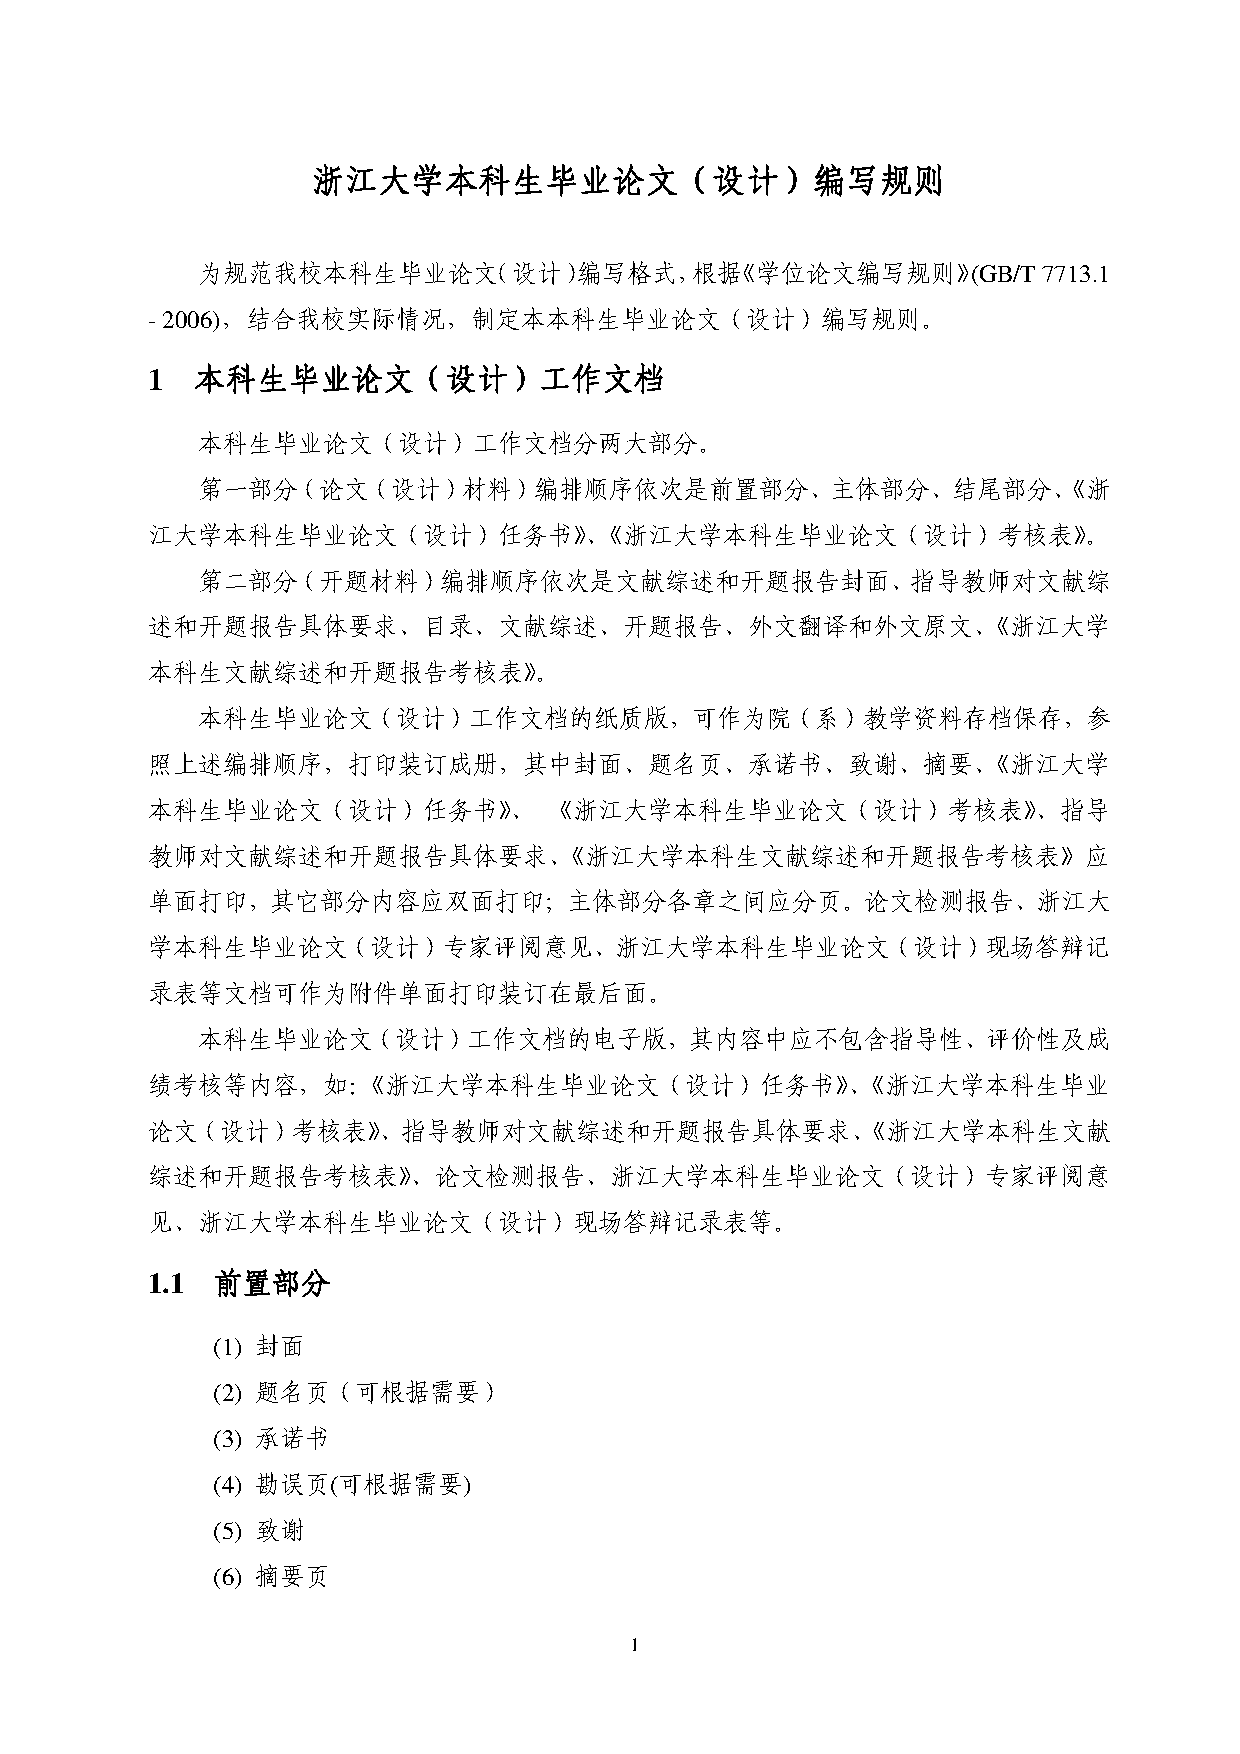
\includepdf[
        pages=1-3,
        scale=0.75,
        pagecommand={\pagestyle{fancy}},
        frame, % remove this line if you don't want outer fram of pdf
    ]{rules2018.pdf}
\end{center}

}
{
    \ifthenelse{\equal{\Type}{design}}
    {
        % `design` content
        %%
% 开题报告
% modifier: 黄俊杰(huangjj27, 349373001dc@gmail.com)
% update date: 2017-05-14

% 选题目的
\objective{

}

% 思路
\methodology{

}

% 研究方法/程序/步骤
\researchProcedure{

}

% 相关支持条件
\supportment{

}

% 进度安排
\schedule{

}

% 指导老师意见
\proposalInstructions{

}


        \cleardoublepage
\chapter{外文翻译}

\section*{摘要}

\section{节标题}

        \cleardoublepage
\chapter{外文原文}

% Insert pdf version of original document
% Place the pdf under `/figure/`

\begin{center}
    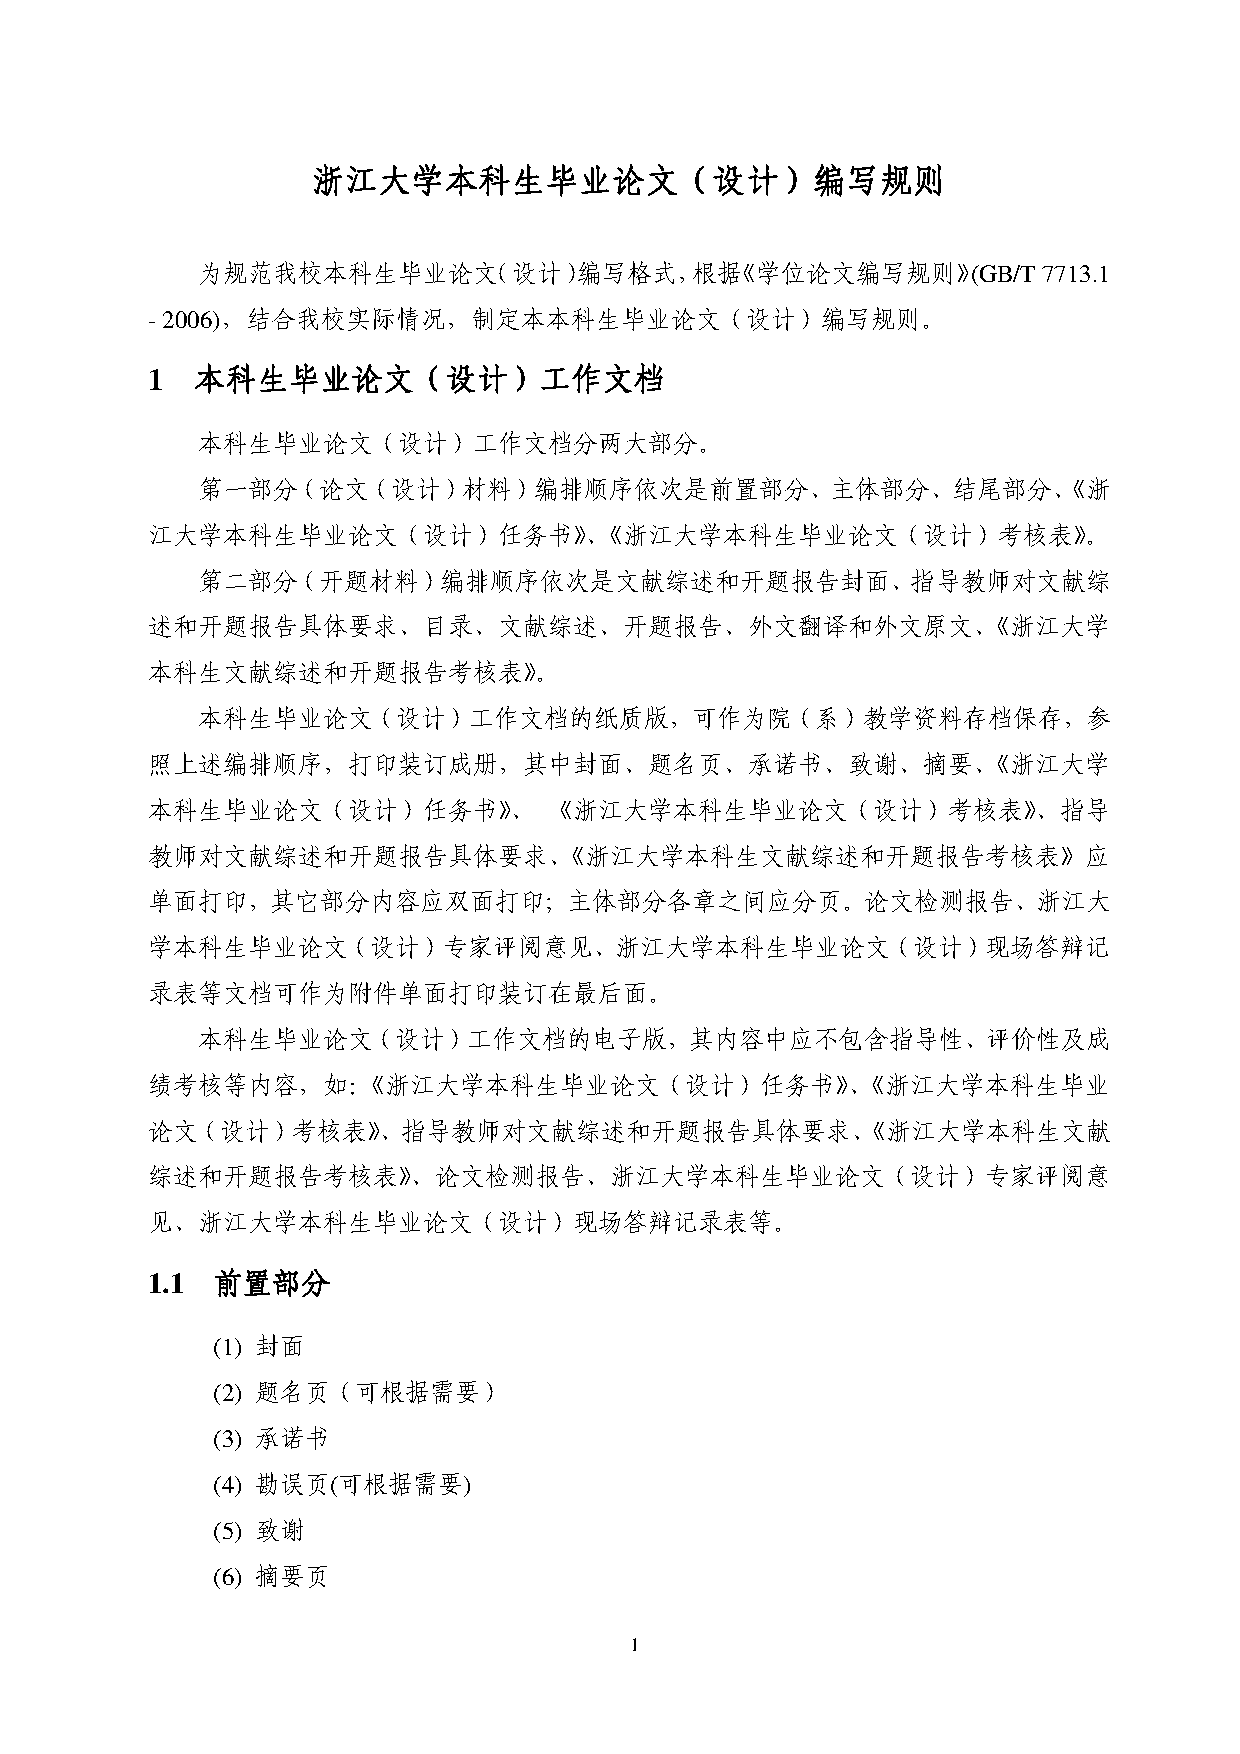
\includepdf[
        pages=1-3,
        scale=0.75,
        pagecommand={\pagestyle{fancy}},
        frame, % remove this line if you don't want outer fram of pdf
    ]{rules2018.pdf}
\end{center}

        \cleardoublepage
\chapter{中期检查}

\section{项目概况}

\section{工作进展情况}

\section{问题与建议}

\section{其他}

    }
    {
        % otherwise, blank
    }
}


% !Mode:: "TeX:UTF-8" 
\begin{conclusions}

学位论文的结论作为论文正文的最后一章单独排写,但不加章标题序号。

结论应是作者在学位论文研究过程中所取得的创新性成果的概要总结,不能与摘要混为一谈。博士学位论文结论应包括论文的主要结果、创新点、展望三部分,在结论中应概括论文的核心观点,明确、客观地指出本研究内容的创新性成果(含新见解、新观点、方法创新、技术创新、理论创新),并指出今后进一步在本研究方向进行研究工作的展望与设想。对所取得的创新性成果应注意从定性和定量两方面给出科学、准确的评价,分(1)、(2)、(3)…条列出,宜用“提出了”、“建立了”等词叙述。

\end{conclusions}
   % 结论
%参考文献

\fancyhead[CO]{\song \xiaowu \leftmark}
\fancyhead[CE]{\song \xiaowu \leftmark}%
\defaultfont

\bibliographystyle{chinesebst2005_UTF8}%
\addcontentsline{toc}{chapter}{参考文献}      % 参考文献加入到中文目录
\addcontentsline{toe}{chapter}{\bfseries  References} % 参考文献加入到英文目录
\addtolength{\bibsep}{-0.8em}
%\nocite{*}
\renewcommand\bibname{参考文献}%book 类
%如果文档类是article之类的, 用\renewcommand\refname{参考文献}
%如果文档类是book之类的, 用\renewcommand\bibname{参考文献}

\bibliography{reference/reference}

%%%%%%%%%%%%%%%%%%%%% appendix.tex %%%%%%%%%%%%%%%%%%%%%%%%%%%%%%%%%
%
% sample appendix
%
% Use this file as a template for your own input.
%
%%%%%%%%%%%%%%%%%%%%%%%% Springer-Verlag %%%%%%%%%%%%%%%%%%%%%%%%%%

\chapter{Chapter Heading}
\label{introA} % Always give a unique label
% use \chaptermark{}
% to alter or adjust the chapter heading in the running head

Use the template \emph{appendix.tex} together with the Springer document class SVMono (monograph-type books) or SVMult (edited books) to style appendix of your book in the Springer layout.


\section{Section Heading}
\label{sec:A1}
% Always give a unique label
% and use \ref{<label>} for cross-references
% and \cite{<label>} for bibliographic references
% use \sectionmark{}
% to alter or adjust the section heading in the running head
Instead of simply listing headings of different levels we recommend to let every heading be followed by at least a short passage of text. Further on please use the \LaTeX\ automatism for all your cross-references and citations.


\subsection{Subsection Heading}
\label{sec:A2}
Instead of simply listing headings of different levels we recommend to let every heading be followed by at least a short passage of text. Further on please use the \LaTeX\ automatism for all your cross-references and citations as has already been described in Sect.~\ref{sec:A1}.

For multiline equations we recommend to use the \verb|eqnarray| environment.
\begin{eqnarray}
\vec{a}\times\vec{b}=\vec{c} \nonumber\\
\vec{a}\times\vec{b}=\vec{c}
\label{eq:A01}
\end{eqnarray}

\subsubsection{Subsubsection Heading}
Instead of simply listing headings of different levels we recommend to let every heading be followed by at least a short passage of text. Further on please use the \LaTeX\ automatism for all your cross-references and citations as has already been described in Sect.~\ref{sec:A2}.

Please note that the first line of text that follows a heading is not indented, whereas the first lines of all subsequent paragraphs are.

% For figures use
%
\begin{figure}[t]
\sidecaption[t]
% Use the relevant command for your figure-insertion program
% to insert the figure file.
% For example, with the graphicx style use
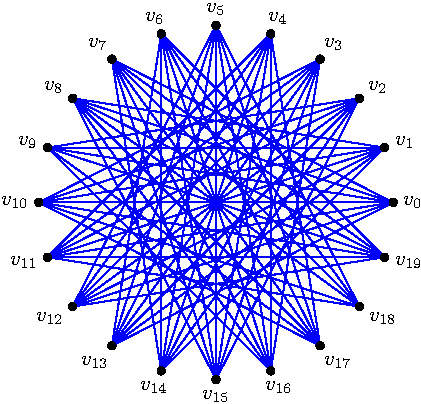
\includegraphics[scale=.65]{figure}
%
% If no graphics program available, insert a blank space i.e. use
%\picplace{5cm}{2cm} % Give the correct figure height and width in cm
%
\caption{Please write your figure caption here}
\label{fig:A1}       % Give a unique label
\end{figure}

% For tables use
%
\begin{table}
\caption{Please write your table caption here}
\label{tab:A1}       % Give a unique label
%
% Follow this input for your own table layout
%
\begin{tabular}{p{2cm}p{2.4cm}p{2cm}p{4.9cm}}
\hline\noalign{\smallskip}
Classes & Subclass & Length & Action Mechanism  \\
\noalign{\smallskip}\hline\noalign{\smallskip}
Translation & mRNA$^a$  & 22 (19--25) & Translation repression, mRNA cleavage\\
Translation & mRNA cleavage & 21 & mRNA cleavage\\
Translation & mRNA  & 21--22 & mRNA cleavage\\
Translation & mRNA  & 24--26 & Histone and DNA Modification\\
\noalign{\smallskip}\hline\noalign{\smallskip}
\end{tabular}
$^a$ Table foot note (with superscript)
\end{table}
%
% 致谢
\defaultfont
\BiAppendixChapter{����\cxueweiѧλ�ڼ�������������} {Papers
Published in the Period of PH. D. Education}

\begin{publist}
\item ����. ��Ŀ. �ڿ�. ��, ��(��): ҳ��

\item ����. ��Ŀ. �ڿ�. ��, ��(��): ҳ��

\item ����. ��Ŀ. �ڿ�. ��, ��(��): ҳ��
\end{publist}
    % 所发文章
\defaultfont

\BiAppendixChapter{��~~~~л}{Acknowledgement}

\ifxueweidoctor               %��ʿҳü
\fancyhead[CO]{\CJKfamily{song}\xiaowu\leftmark}
\else
\fancyhead[CO]{\CJKfamily{song}\xiaowu ��������ҵ��ѧ\cxueke \cxuewei ѧλ����}
\fi
\fancyhead[CE]{\CJKfamily{song}\xiaowu ��������ҵ��ѧ\cxueke \cxuewei ѧλ���� }%

������ģ����UFO@bbs.hit.edu.cn�ġ���������ҵ��ѧ��ѧ��ʿ��˶ʿ������ģ�塷�Ļ����ϣ�
���ںܶ��˵İ�������ɵģ��ڴ�һ�������DZ�ʾ��л��

�ر��лStanley����������ģ�忪Դ��ĿPluto�Լ���������ģ��Ĵ����޸ģ�
ʹ֮���ӷ��Ϲ�������ģ��Ҫ��

�ر��л�������϶���վ��~Tex~�İ���~Tex��nebula������cucme��
������ʼ���ն�ȫ��֧��ģ�����������Ϊ�����˴����Ĺ�����

��л���괺~(HIT bbs ID: dengnch)�������˴�����ʱ��������ģ���
һϵ�в�����ʹ�ø�~\LaTeX~ģ��Ͷ�Ӧ��~Word~ģ��ĸ�ʽ������ȫһ�¡�

��лˮľ�廪��~\TeX~��~\LaTeX~��ĸ�λ����Ϊ���ṩ�ĸ��ְ�����
�ر���~snoopyzhao~���ѣ���������ĵ�Ϊ��ģ�����������ѣ�ʹ��ģ�����������
˳�����С�

������ĸ�л�������϶���~bbs~վ~Tex~���������ѵĴ���֧�֣�



ֵ���������֮�ʣ������������˽��������ʦ��ͬѧ�����Գ�ֿ��л�⣡

���ȸ�л�ҵĵ�ʦ{\bf ijijij}���ڣ������ĵ��о�����������{\bf
ij}��ʦ����Ľ�����չ���ġ�
����ѧ���ϲ��Ͻ�ȡ������������ִ��׷��ľ�������ѧϰ�İ�����{\bf
ij}��ʦ��������̵���ʶ������dz���Ľ�������������ӡ��


��л{\bf ijijij}���ں�{\bf ijijij}���ڶ���ѧϰ�͹����İ�����
�����ڷܵĹ������硢��۵�����̬�ȶ�����ظ�Ⱦ���ҡ���л{\bf
ijijij}���ں�{\bf ijijij}���ڶ���ѧҵ�������ϵĹ��ġ�


��л��ʿ��{\bf ijijij}��{\bf ijijij}��{\bf ijijij}��{\bf ijijij}��
���ҵ���˽�����ͻ���֧�֡���лʵ�������е��ֵܽ����ǣ�
����Ҷȹ����ⳤ�õ�ѧϰ���о��׶Σ������ҽ�����⣬����˼�롣

����ر�Ҫ��л�ҵ������ǣ����Ƕ���Ҫ�����٣��������ҵĶ��ǹػ���֧�ֺ����⡣
% 致谢
%!Tex Program = xelatex
% -*-coding: utf-8 -*-
\pagestyle{empty}
\newcommand{\subchapterstyle}%
  {\song\rmfamily\bfseries\xiaoer}  
\addcontentsline{toc}{chapter}{独创性声明}
\begin{center}{\subchapterstyle 独创性声明}\end{center}

 本人声明所呈交的学位论文是本人在导师指导下进行的研究工作及取得的研
 究成果。据我所知,除了文中特别加以标注和致谢的地方外,论文中不包含其他
 人已经发表或撰写过的研究成果,也不包含为获得\underline{\textbf{~东北林业大学~}}或其他教育
 机构的学位或证书而使用过的材料。与我一同工作的同志对本研究所做的任何贡献均己在论文中作了明确的说明并表示谢意

\vspace{\baselineskip}
\hspace{4em}学位论文作者签名:\hfill 签字日期:\hspace{2.5em}年\hspace{1.5em}月\hspace{1.5em}日

\vspace{2\baselineskip}
\addcontentsline{toc}{chapter}{学位论文版权使用授权书}
\begin{center}{\subchapterstyle 学位论文版权使用授权书}\end{center}

本学位论文作者完全了解\underline{\textbf{~东北林业大学~}}有关保留、使用学位论文的规
定,有权保留并向国家有关部门或机构送交论文的复印件和磁盘,允许论文被查
阅和借阅。本人授权\underline{\textbf{~东北林业大学~}}可以将学位论文的全部或部分内容编入有
关数据库进行检索,可以采用影印、缩印或扫描等复制手段保存、汇编学位论
文。
(保密的学位论文在解密后适用本授权书)

%\vspace{\baselineskip}
%本学位论文属于(请在以下相应方框内打“$\surd$”):
%
%保密\xiaoer$\square$\xiaosi ,在~~~~~~~~~~~~~年解密后适用本授权书
%
%不保密\xiaoer$\square$\xiaosi

\vspace{\baselineskip}
\hspace{4em}学位论文作者签名:\hfill 签字日期:\hspace{2.5em}年\hspace{1.5em}月\hspace{1.5em}日

\vspace{\baselineskip}
\hspace{4em}导师签名:\hfill 签字日期:\hspace{2.5em}年\hspace{1.5em}月\hspace{1.5em}日

\vspace{2\baselineskip}
学位论文作者毕业后去向:\\

\vspace{\baselineskip}
\hspace{4em}工作单位:  \hfill 电话:

\vspace{\baselineskip}
\hspace{4em}通讯地址:  \hfill  邮编:

   % 承诺

\clearpage


\end{document}
